\section{User Manual}
\label{sec:user-manual}

\subsection{Manual Guide for Submitting Expense Reports}

\begin{enumerate}
    \item Log in with your corporate email account.

    \begin{figure}[H]
        \centering
        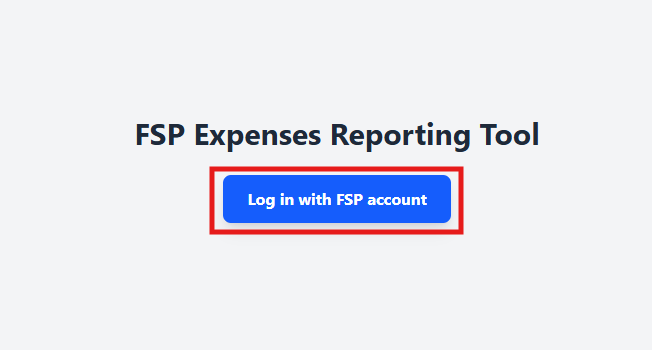
\includegraphics[width=0.8\textwidth]{Images/UserManual/image12.png}
        \caption[Application login view]
        {Application login view. [Own creation]}
        \label{fig:application-login-screen}
    \end{figure}

    \item Upload one or multiple expenses through one of the following methods:
    \begin{enumerate}[label=\alph*)]
        \item Drag and drop receipt files directly into the application.
            
        \begin{figure}[H]
            \centering
            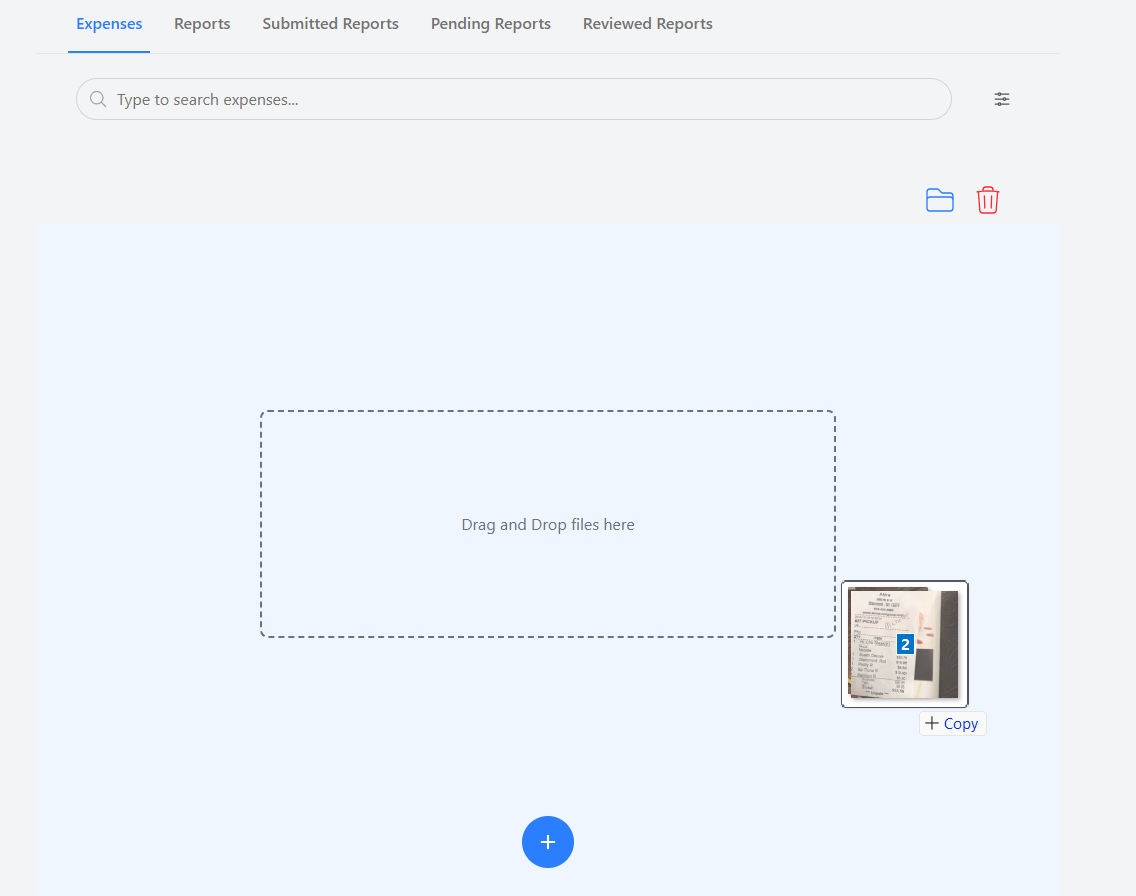
\includegraphics[width=0.8\textwidth]{Images/UserManual/image8.png}
            \caption[Uploading expenses via drag-and-drop interface]
            {Uploading expenses via drag-and-drop interface. [Own creation]}
            \label{fig:drag-and-drop-upload}
        \end{figure}

        \item Click on the add icon button located at the bottom center of the screen to open the file browser and select the receipts to upload.
            
        \begin{figure}[H]
            \centering
            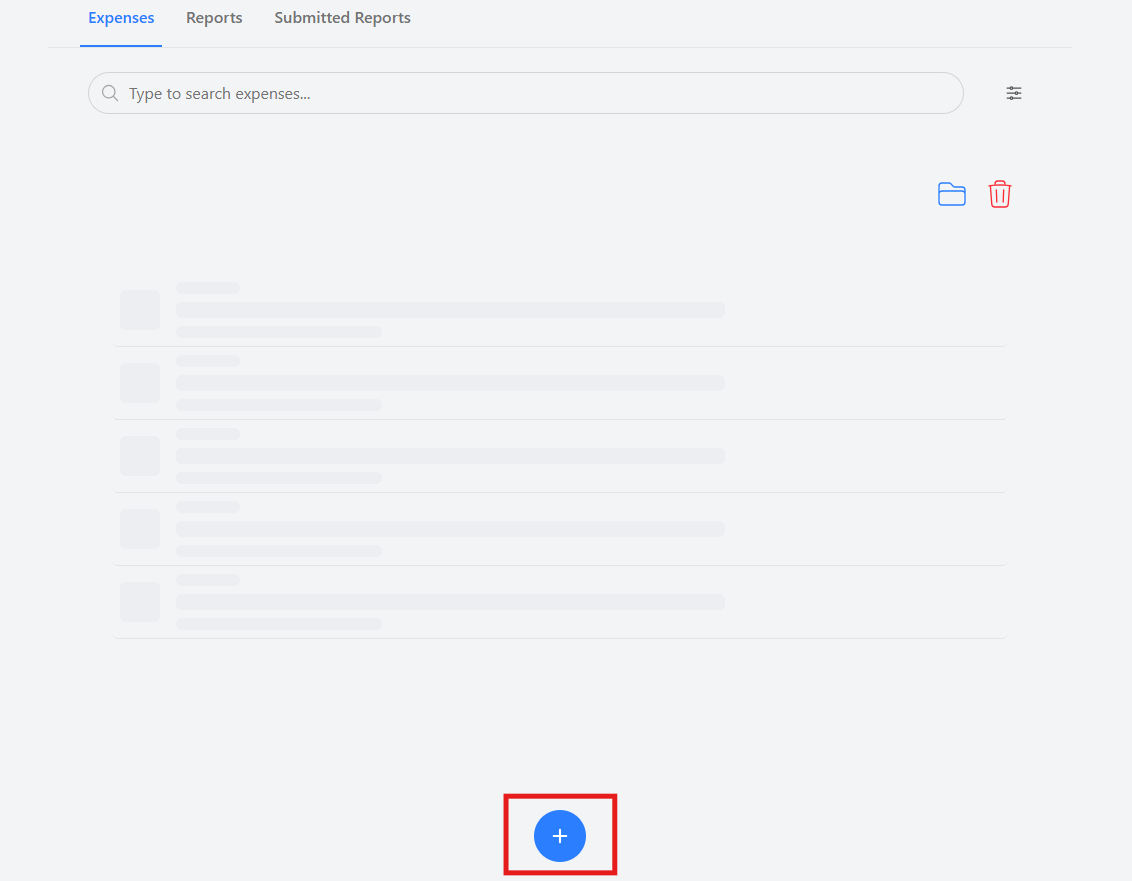
\includegraphics[width=0.75\textwidth]{Images/UserManual/image15.png}
            \caption[Uploading expenses from file browser]
            {Uploading expenses from file browser. [Own creation]}
            \label{fig:file-browser-upload}
        \end{figure}

    \end{enumerate}

    \item Wait until the expense is completely processed by the AI model (i.e., when the expense status changes from \textit{Processing} to another status).

    \begin{figure}[H]
        \centering
        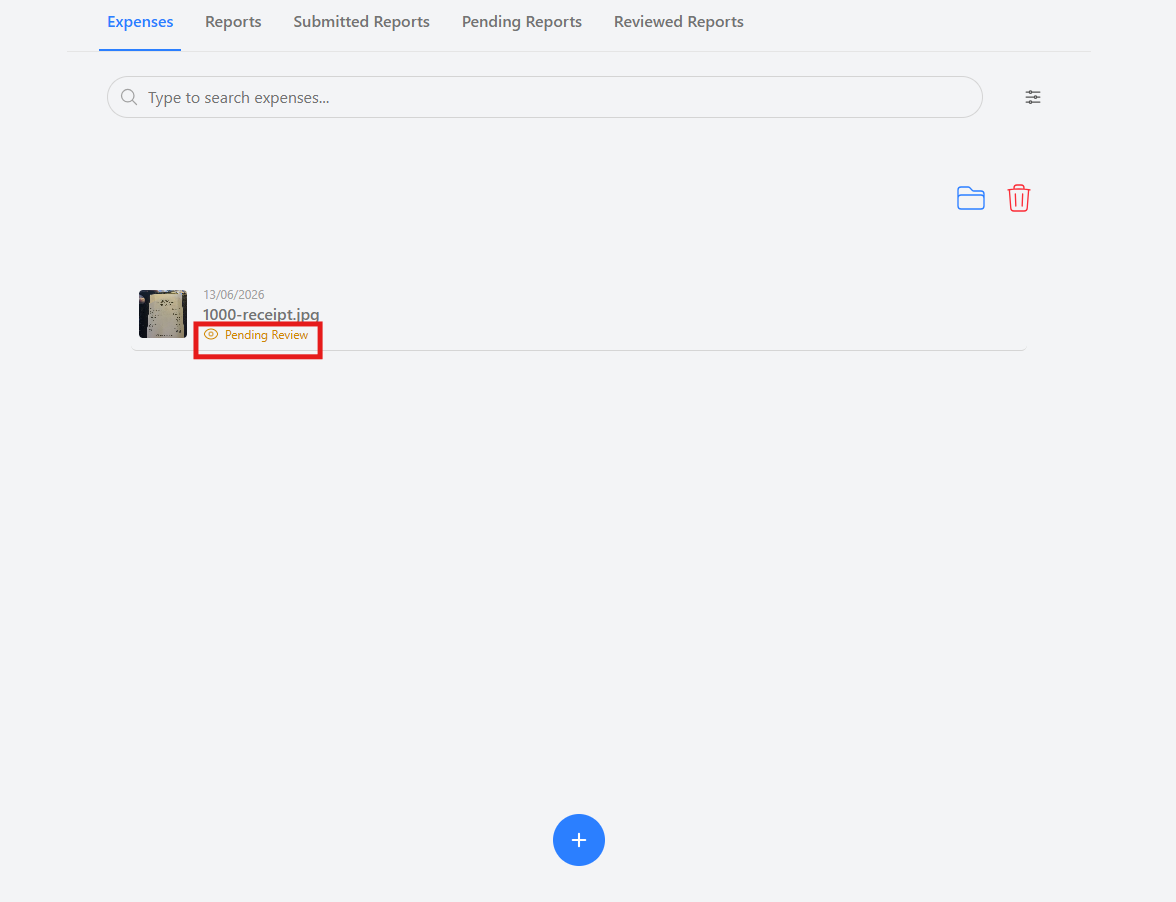
\includegraphics[width=0.8\textwidth]{Images/UserManual/image17.png}
        \caption[Expense status after AI extraction]
        {Expense status after AI extraction. [Own creation]}
        \label{fig:expense-status-after-AI-extraction}
    \end{figure}

    \item Click on the uploaded expense and review or correct the AI-extracted information. Fill in any missing required data. To save the updated expense information, click the \textit{Save} button.

    \begin{figure}[H]
        \centering
        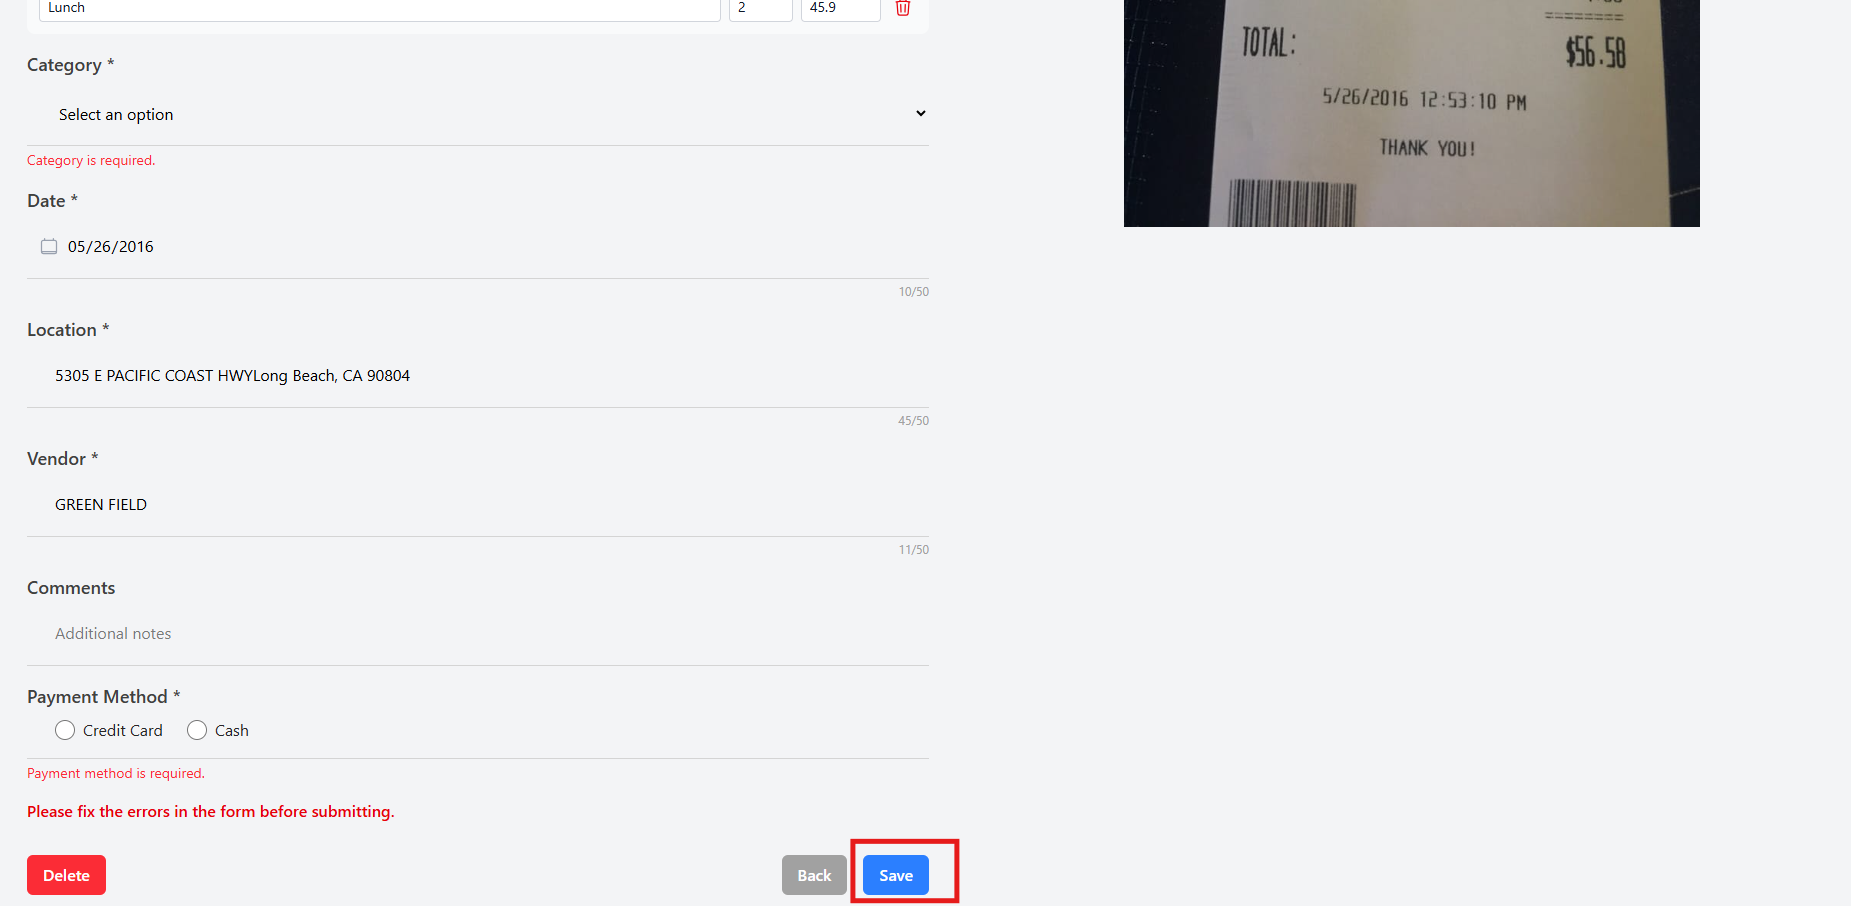
\includegraphics[width=0.8\textwidth]{Images/UserManual/image5.png}
        \caption[Expense detail view for reviewing AI-extracted data]
        {Expense detail view for reviewing AI-extracted data. [Own creation]}
        \label{fig:expense-detail-view}
    \end{figure}

    \item Once the expense has been manually reviewed (showing the \textit{Reviewed} status), it is ready to be attached to a report.

    \begin{figure}[H]
        \centering
        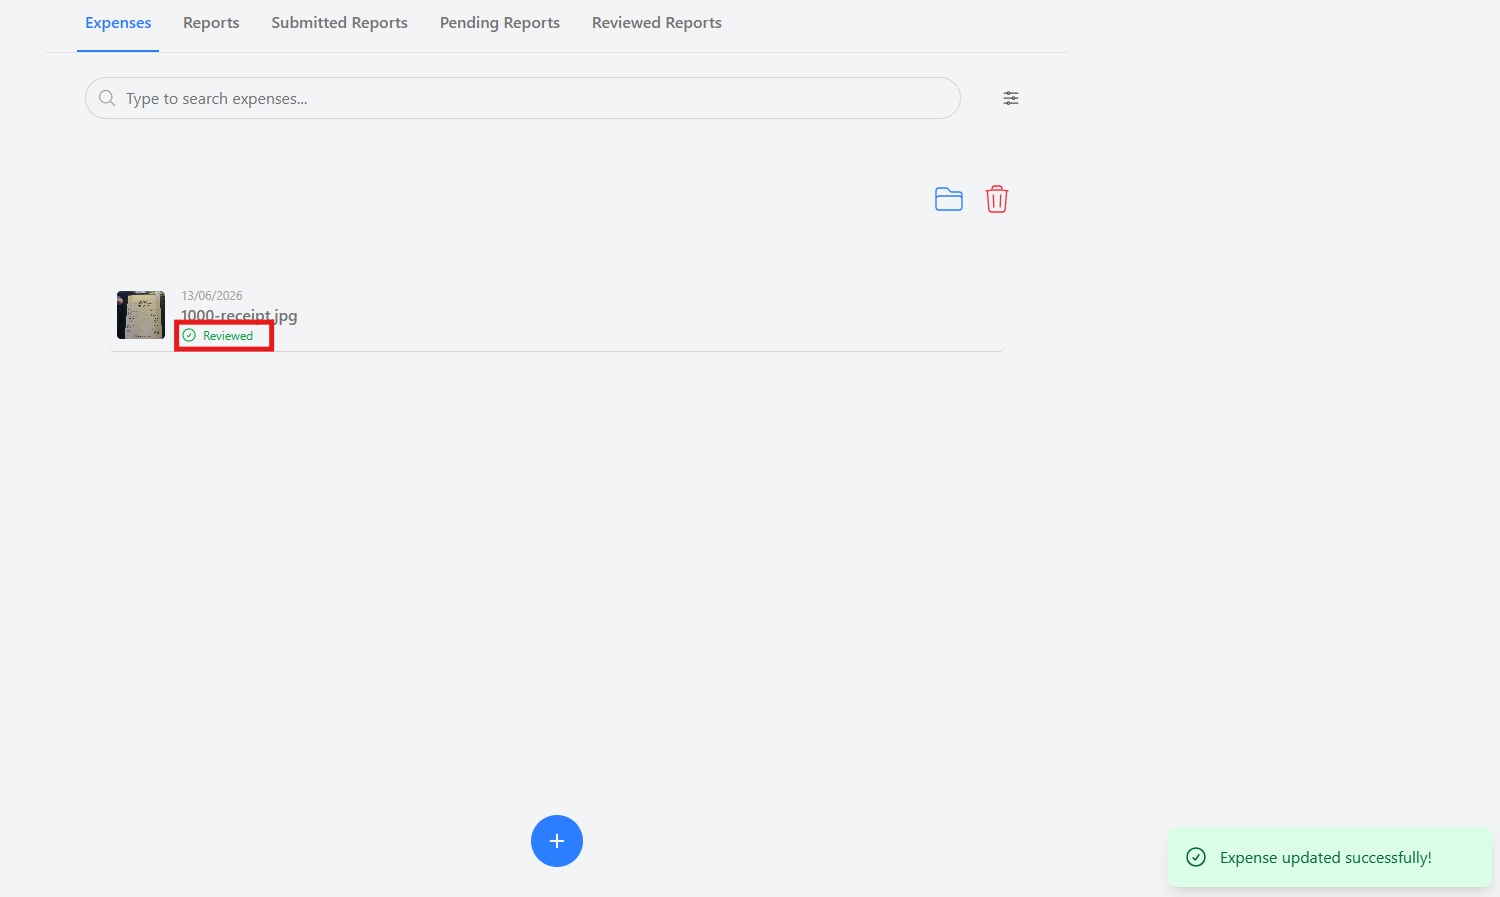
\includegraphics[width=0.8\textwidth]{Images/UserManual/image2.png}
        \caption[Expense status after manual review]
        {Expense status after manual review. [Own creation]}
        \label{fig:expense-status-after-review}
    \end{figure}

    \newpage

    Only expenses with \textit{Reviewed} status can be attached to a report using one of the following methods:

    \begin{enumerate}[label=\alph*)]
        \item Click on the folder icon to select expenses with \textit{Reviewed} status.

        \begin{figure}[H]
            \centering
            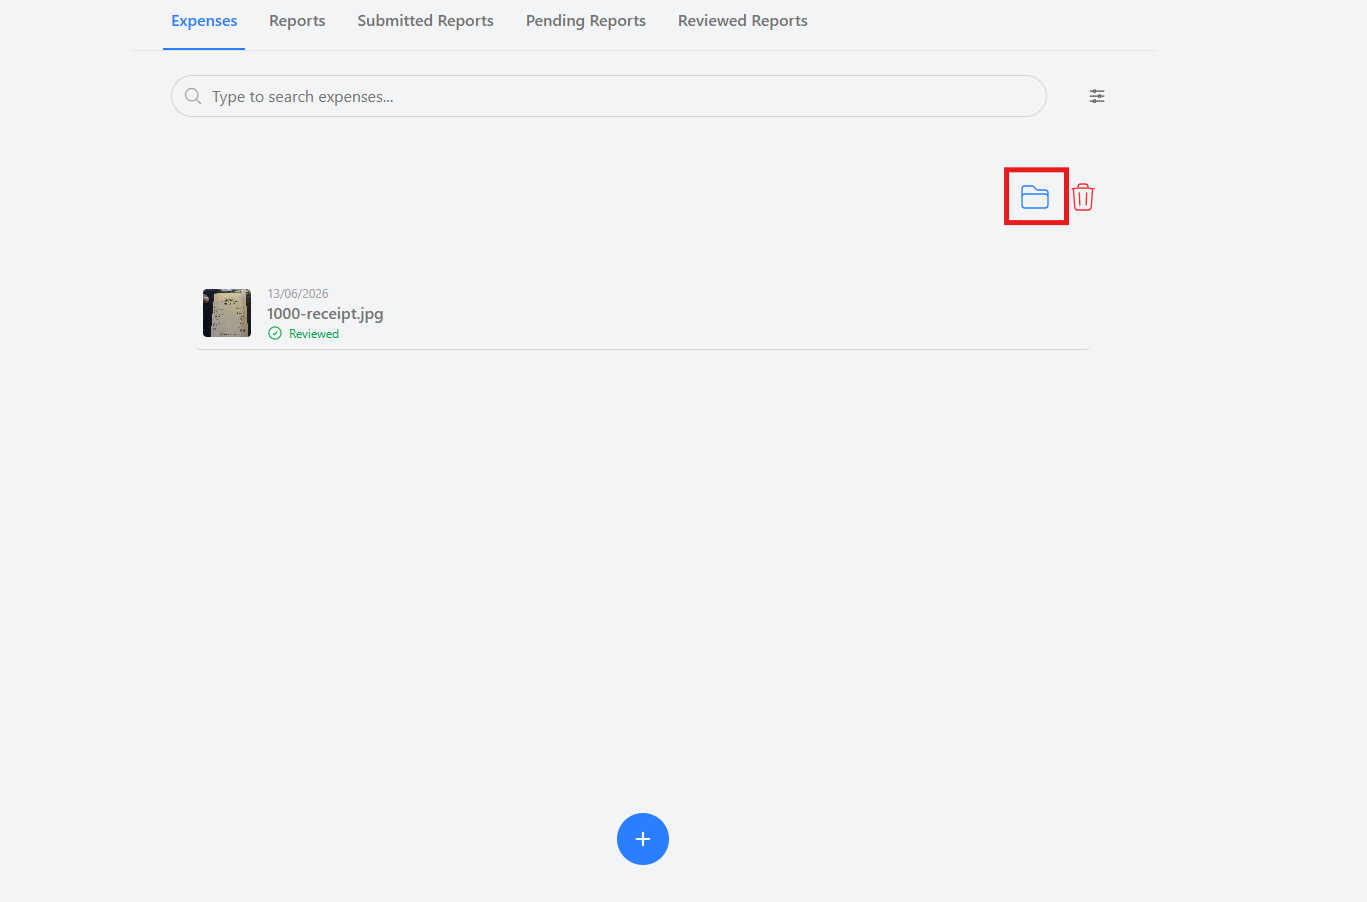
\includegraphics[width=0.8\textwidth]{Images/UserManual/image3.png}
            \caption[Toggle button for attaching expenses to report]
            {Toggle button for attaching expenses to report. [Own creation]}
            \label{fig:toggle-button-attach-expenses}
        \end{figure}

        Select the expenses you want to attach to a report and assign them to either a new or an existing report. If creating a new report, a dialogue similar to Figure \ref{fig:new-report-dialogue} will appear, where you can complete all required information.

        
        \begin{figure}[H]
            \centering
            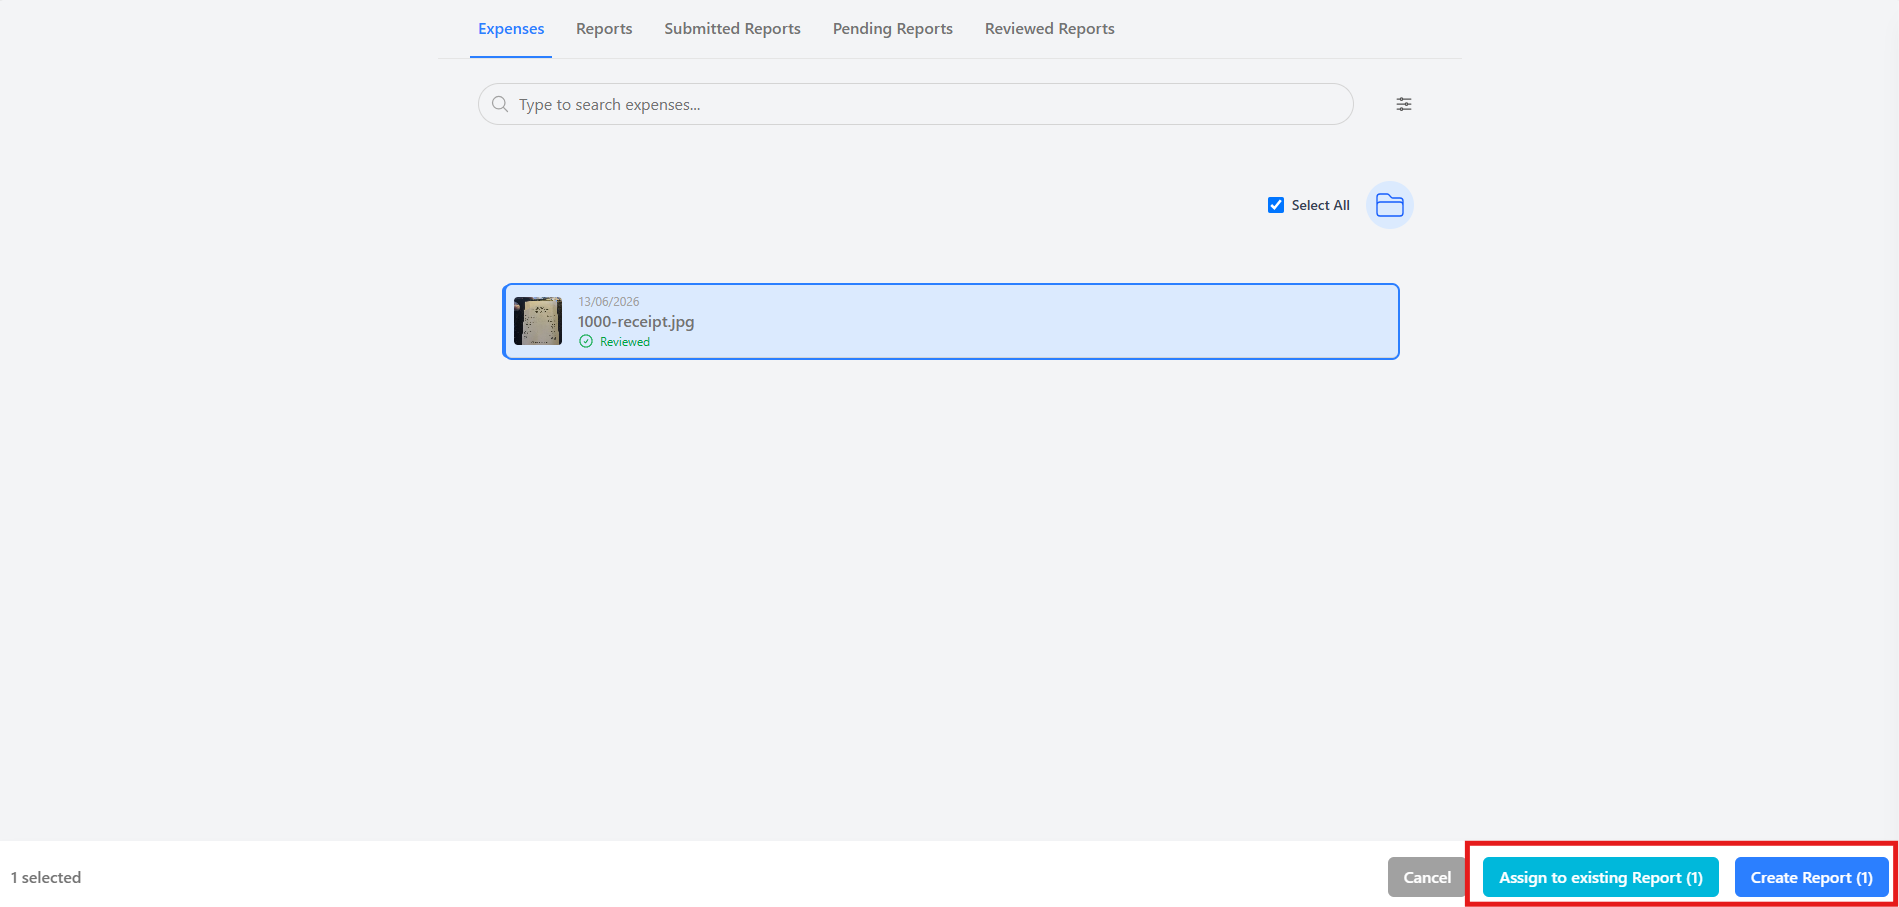
\includegraphics[width=0.8\textwidth]{Images/UserManual/image9.png}
            \caption[Options for attaching selected expenses to report]
            {Options for attaching selected expenses to report. [Own creation]}
            \label{fig:options-attach-expenses}
        \end{figure}

        \vspace{4cm}

        \item Create a new report from the \textit{Reports} view.
            
                Fill in the required information for creating a new report.

            
        \begin{figure}[H]
            \centering
            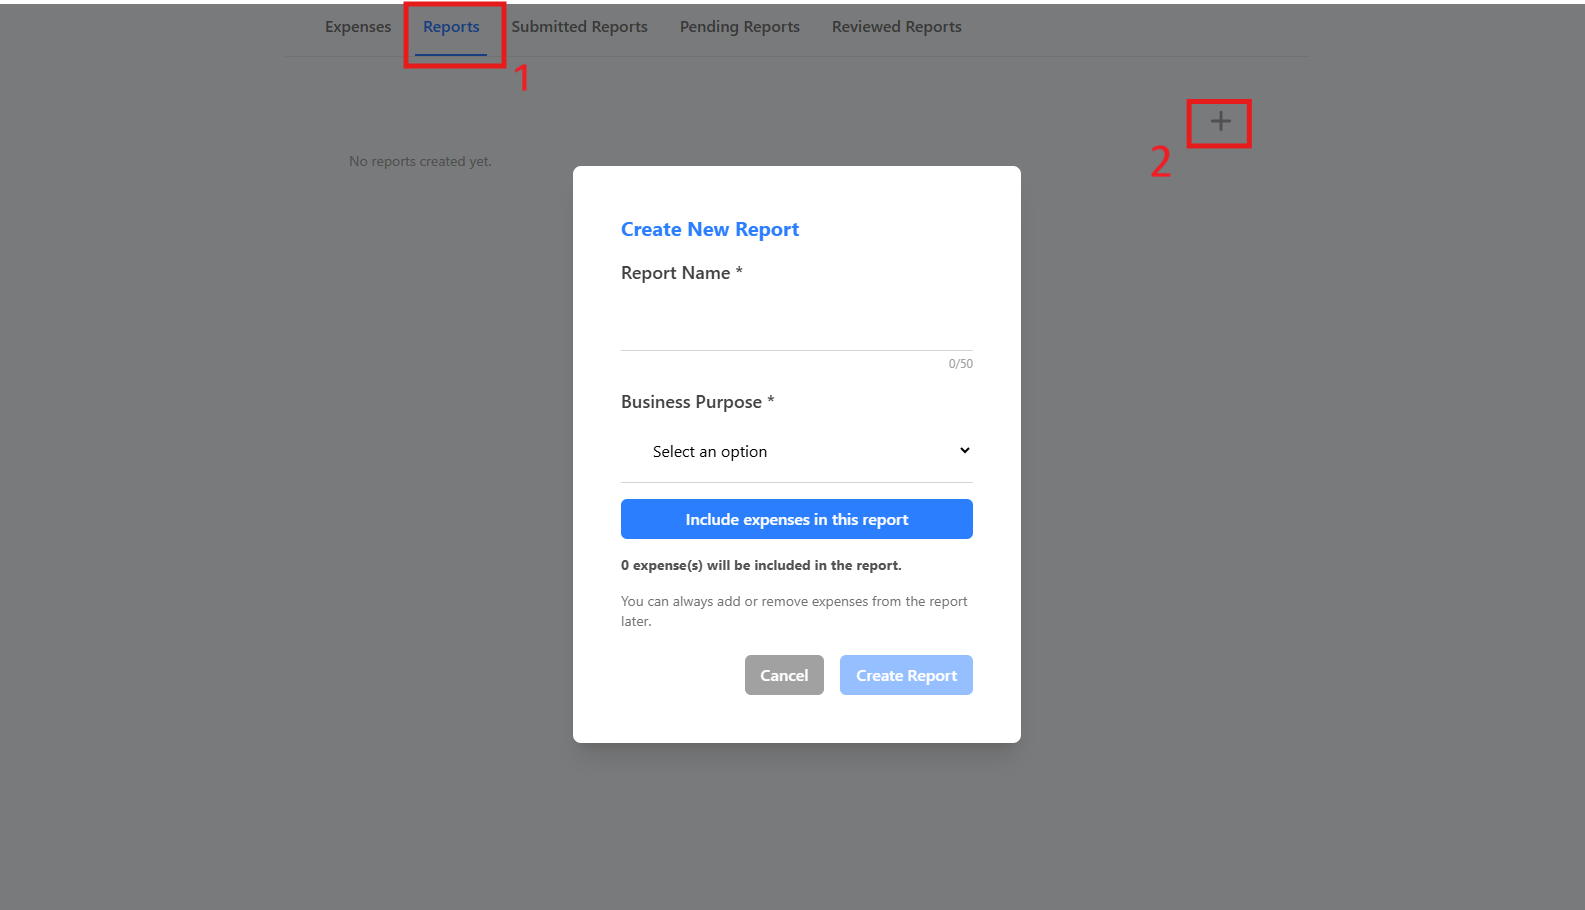
\includegraphics[width=0.8\textwidth]{Images/UserManual/image14.png}
            \caption[Creating new report from Reports view]
            {Creating new report from Reports view. [Own creation]}
            \label{fig:new-report-dialogue}
        \end{figure}


        Click on the new report and assign expenses with “Reviewed” status to the existing report.

        \begin{figure}[H]
            \centering
            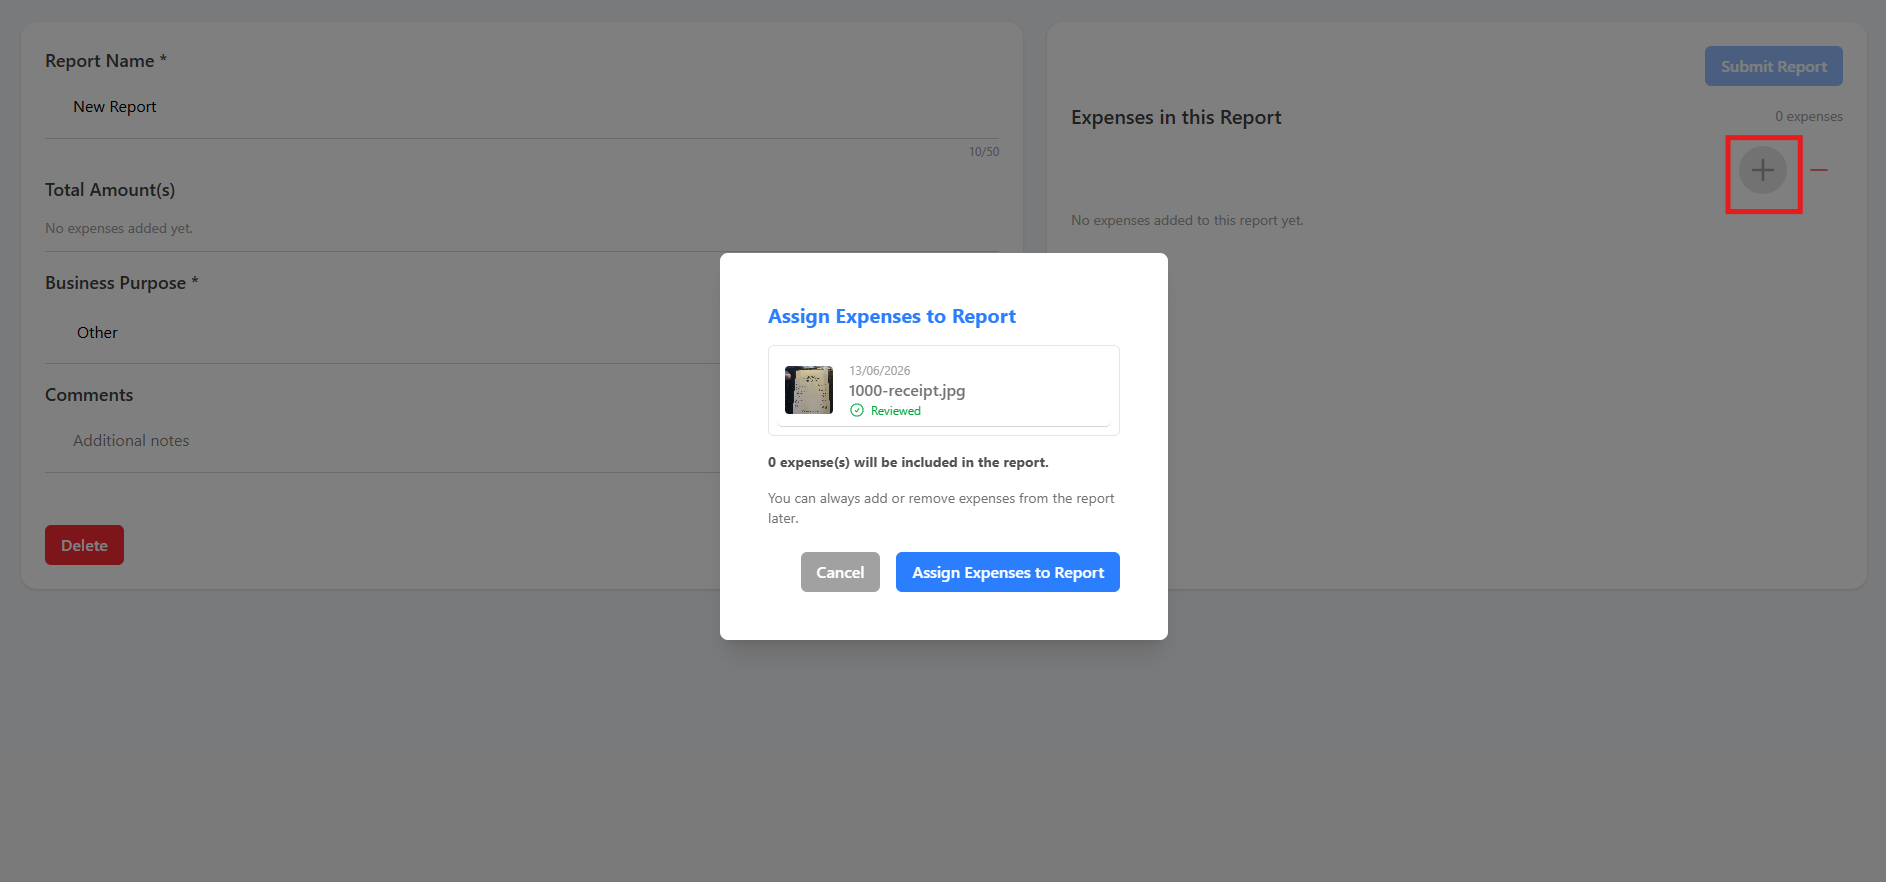
\includegraphics[width=0.8\textwidth]{Images/UserManual/image11.png}
            \caption[Dialogue for assigning expenses to report]
            {Dialogue for assigning expenses to report. [Own creation]}
            \label{fig:assign-expenses-to-current-report}
        \end{figure}
        
    \end{enumerate}

    \item Click on the report to review and correct its information, then press the \textit{Save Changes} button to save the updated report information successfully.


    \begin{figure}[H]
        \centering
        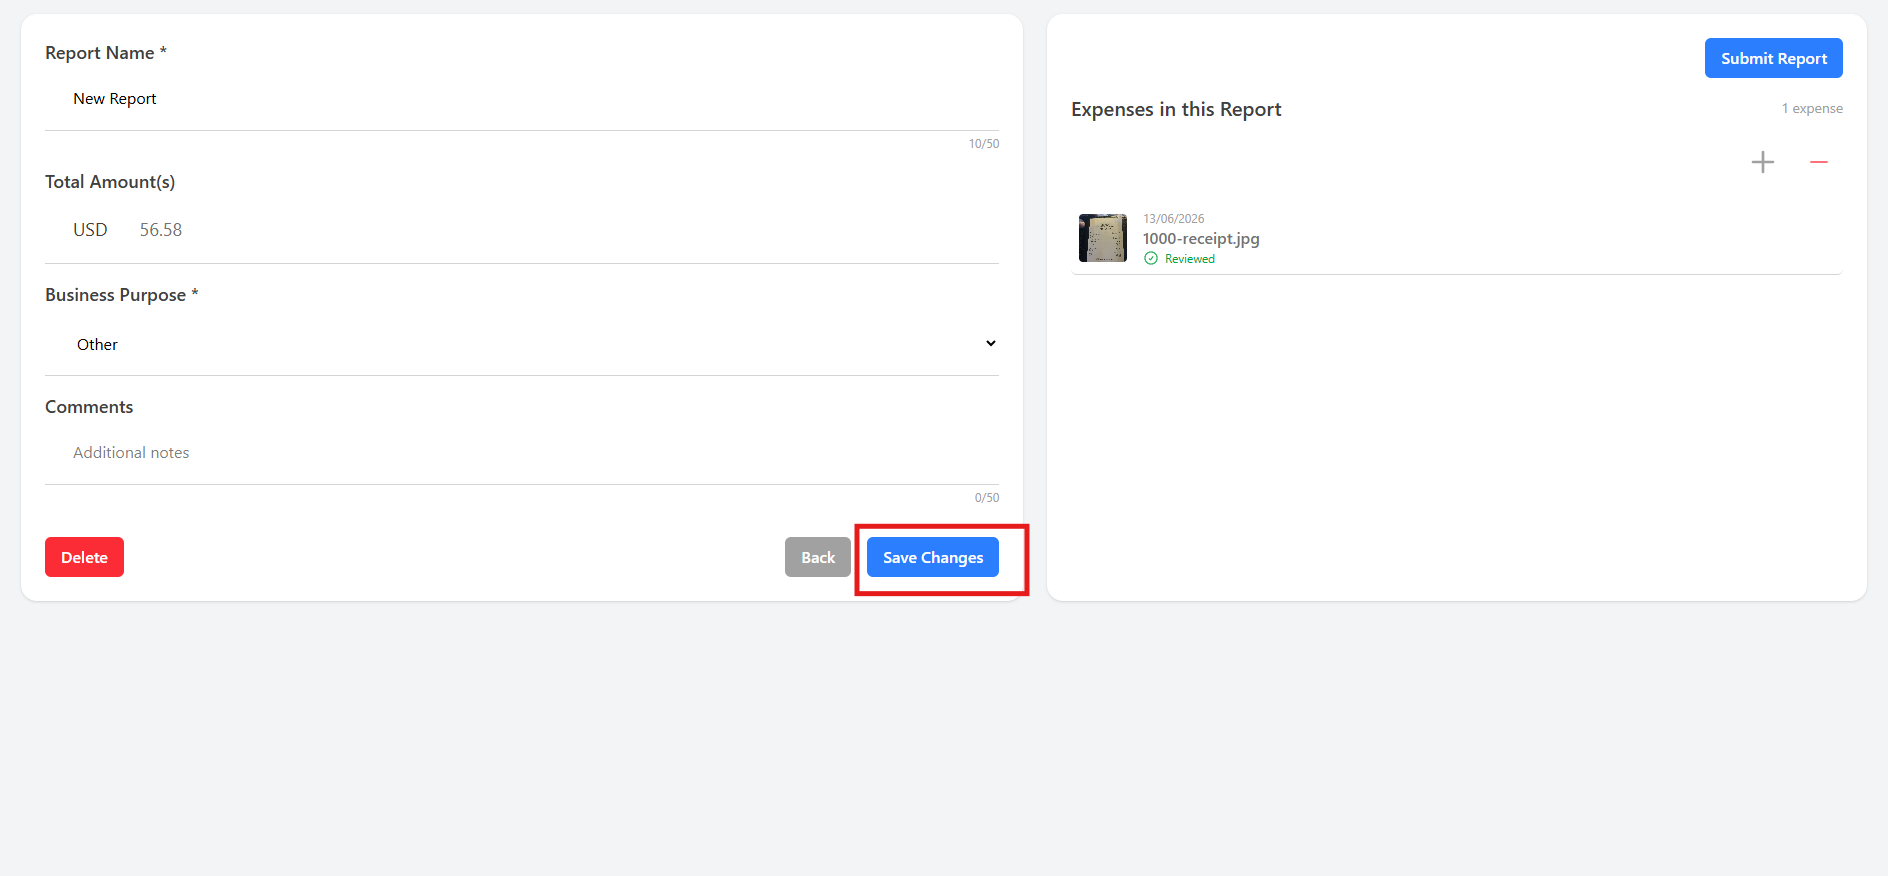
\includegraphics[width=0.8\textwidth]{Images/UserManual/image13.png}
        \caption[Report detail view for reviewing information]
        {Report detail view for reviewing information. [Own creation]}
        \label{fig:report-detail-view}
    \end{figure}


    Attachment or detachment of expenses is also possible by clicking the add or minus icons.


    \begin{figure}[H]
        \centering
        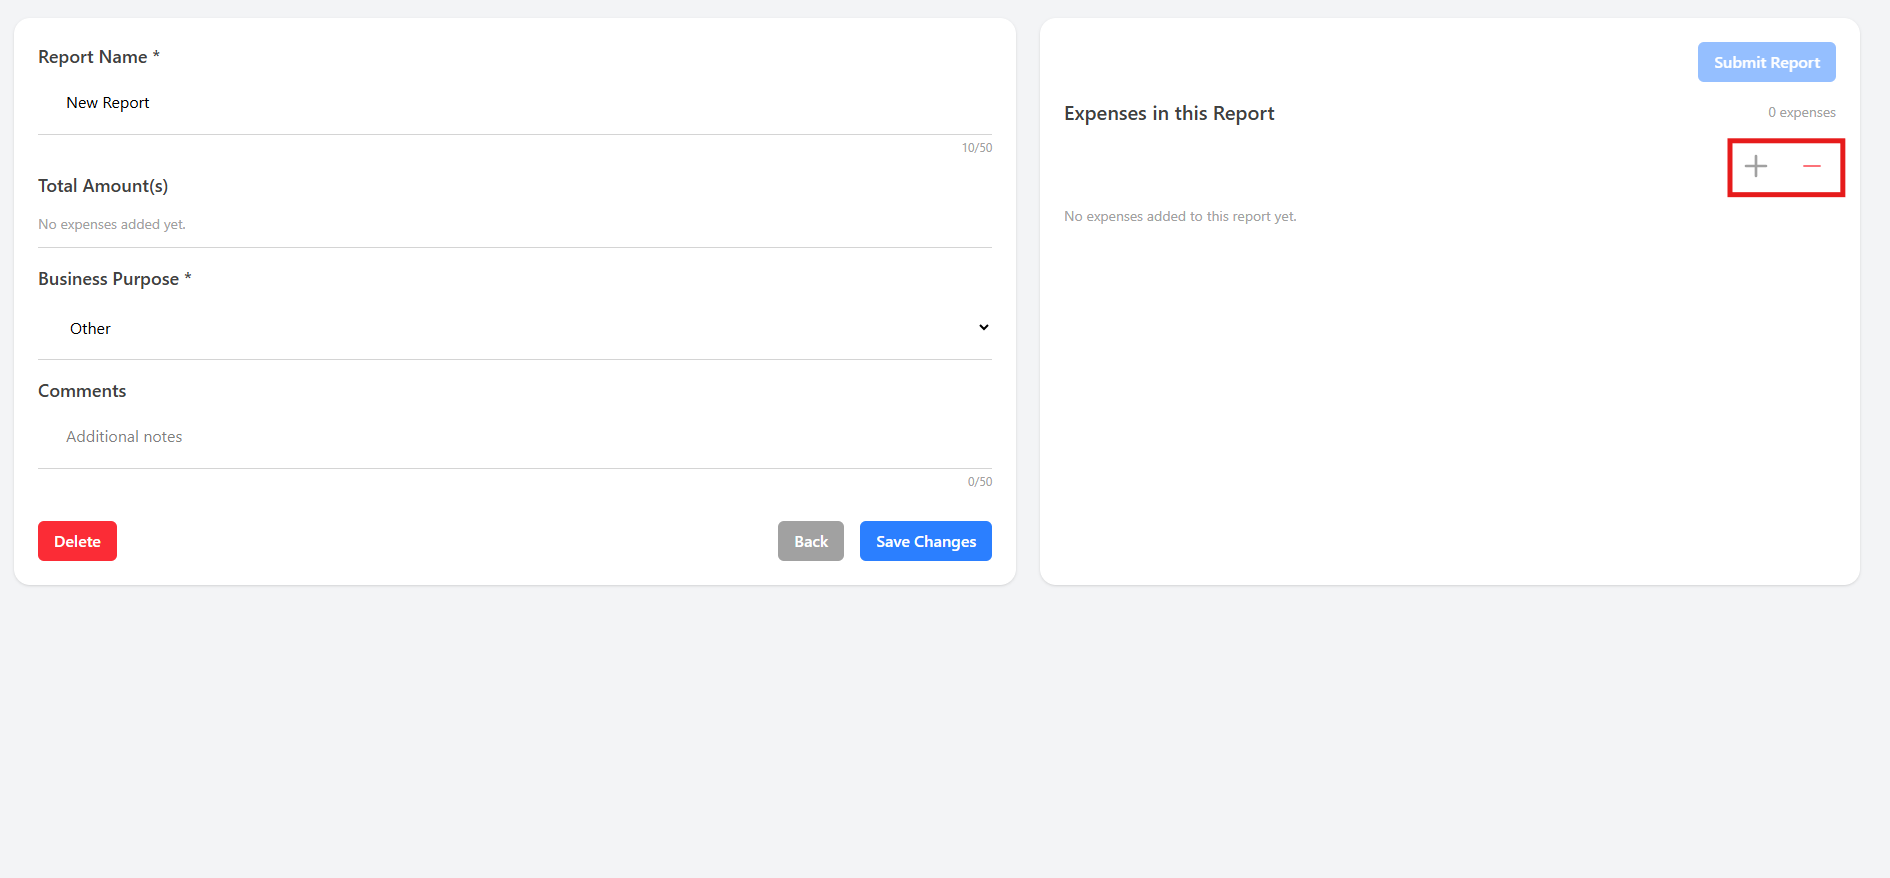
\includegraphics[width=0.8\textwidth]{Images/UserManual/image18.png}
        \caption[Options for attaching or detaching expenses from report]
        {Options for attaching or detaching expenses from  report. [Own creation]}
        \label{fig:attach-detach-expenses}
    \end{figure}


    \item Once the report is ready for submission, click the \textit{Submit} button.

    \begin{figure}[H]
        \centering
        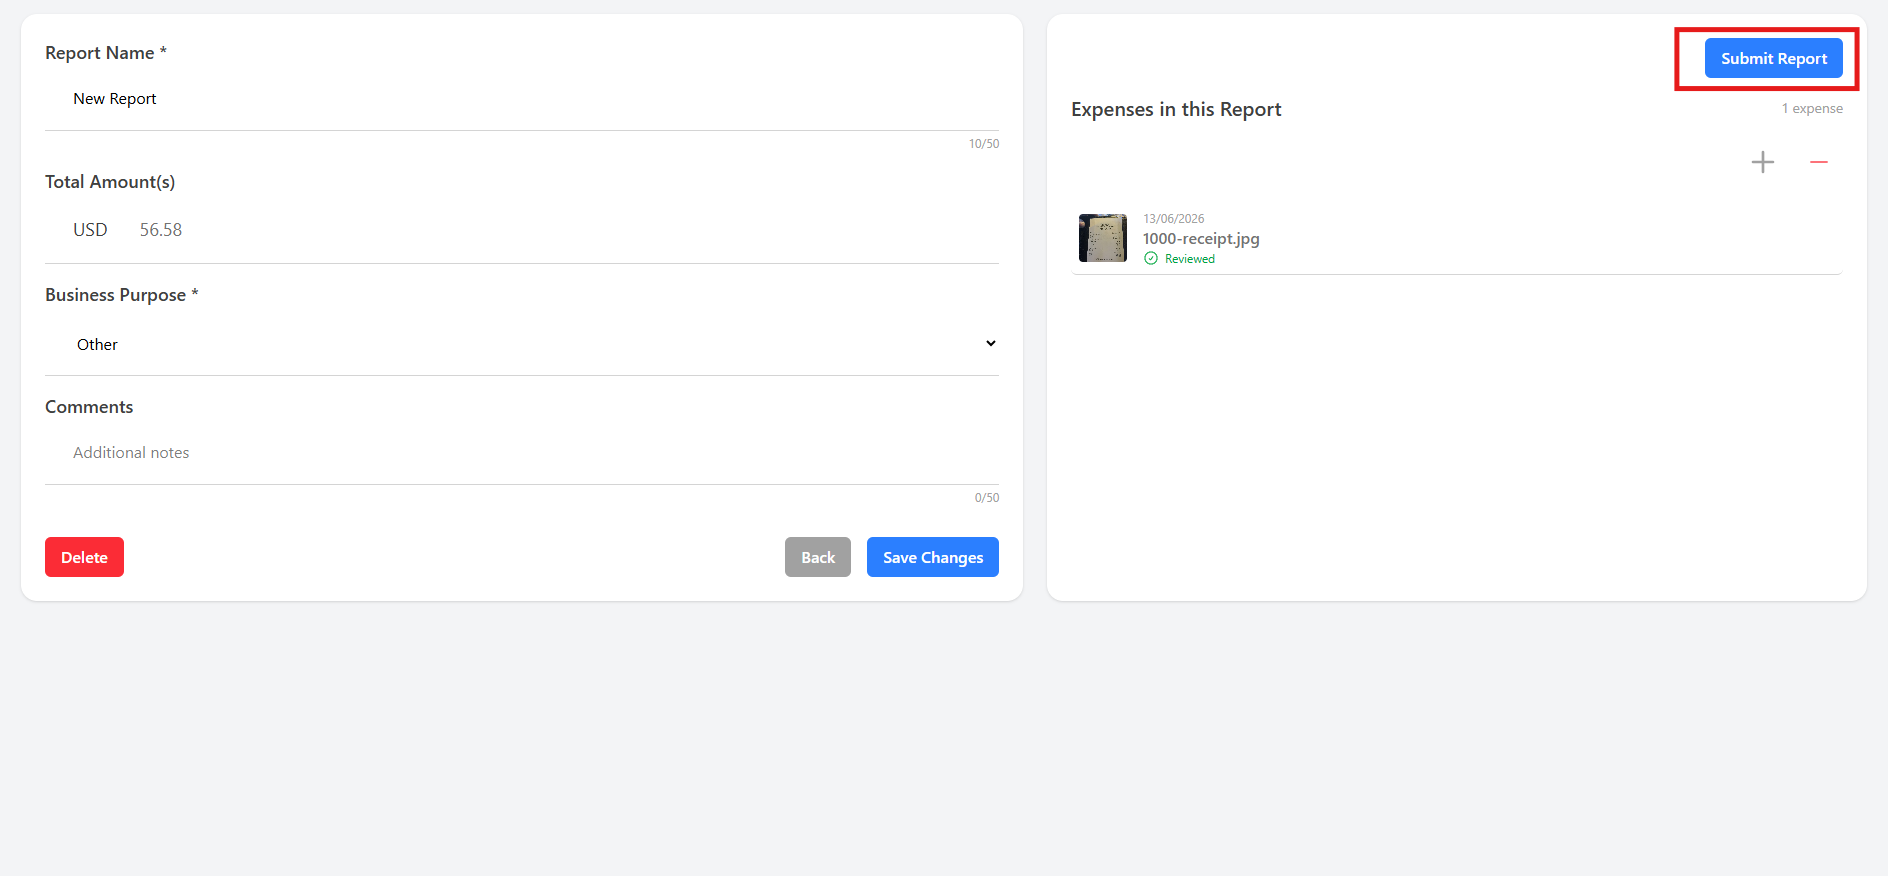
\includegraphics[width=0.8\textwidth]{Images/UserManual/image1.png}
        \caption[Submit report button]
        {Submit report button. [Own creation]}
        \label{fig:submit-report}
    \end{figure}

    \item After the report has been submitted, you can view its real-time status on the \textit{Submitted Reports} view.


    \begin{figure}[H]
        \centering
        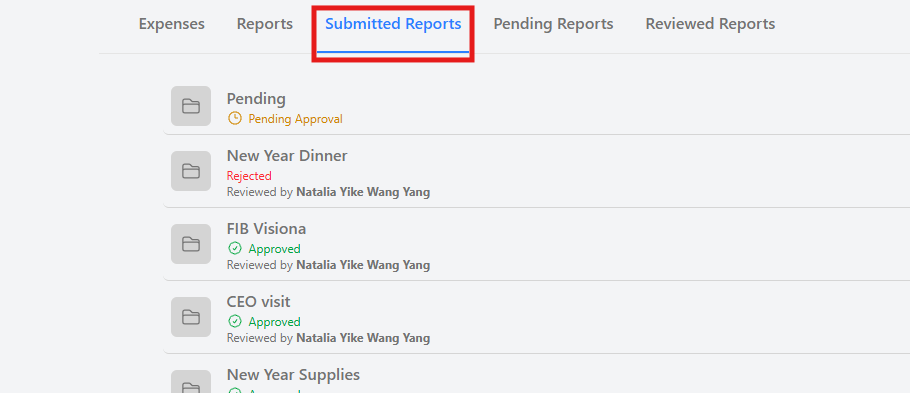
\includegraphics[width=0.8\textwidth]{Images/UserManual/image4.png}
        \caption[Submitted Reports view]
        {Submitted Reports view. [Own creation]}
        \label{fig:submitted-reports}
    \end{figure}

\end{enumerate}

%manual admin

\subsection{Manual Guide for Reviewing Expense Reports}

\begin{enumerate}
    \item View reports pending review by selecting the \textit{Pending Reports} option from the upper screen tab.

    \begin{figure}[H]
        \centering
        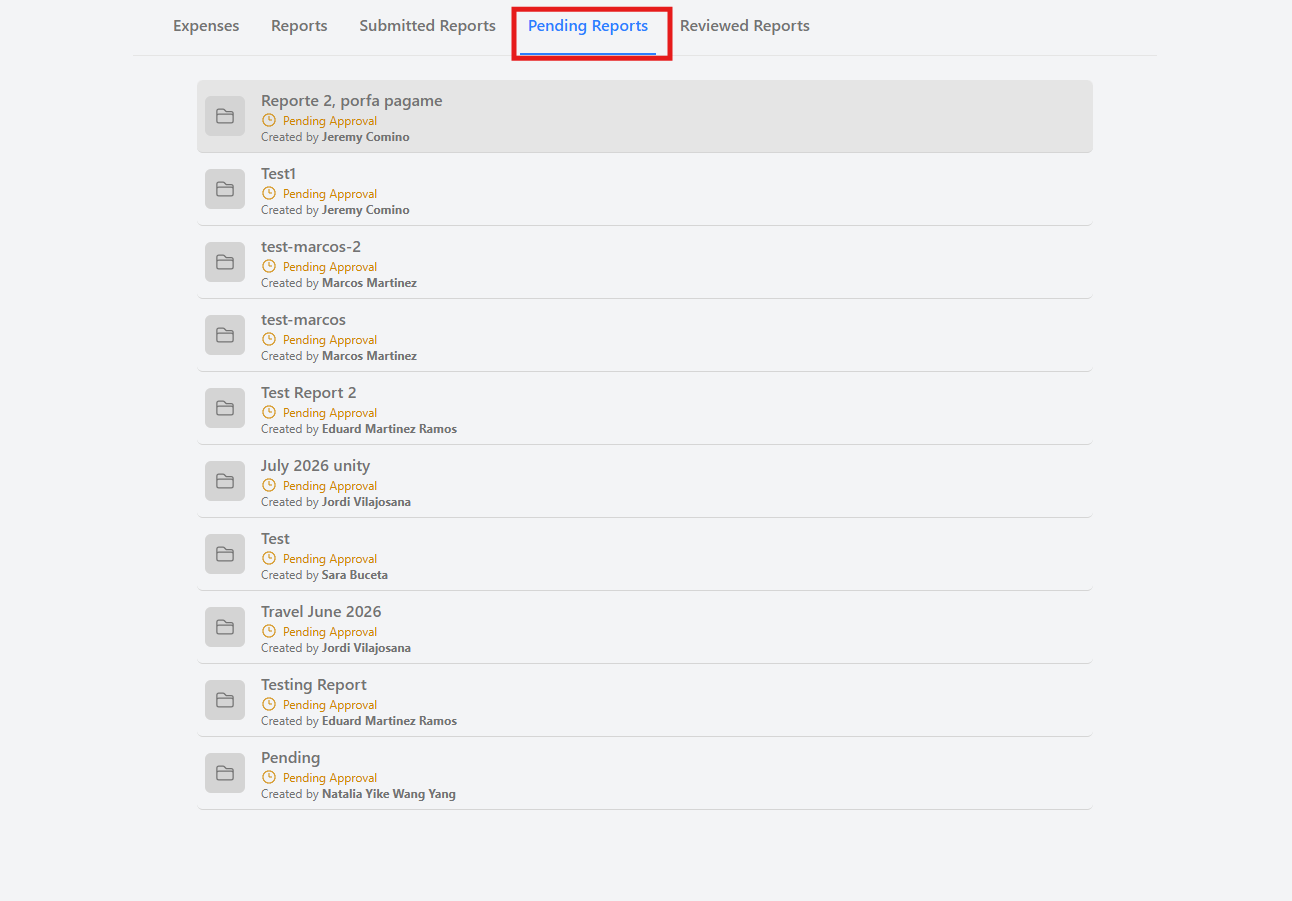
\includegraphics[width=0.8\textwidth]{Images/UserManual/image10.png}
        \caption[Pending Reports view]
        {Pending Reports view. [Own creation]}
        \label{fig:pending-reports}
    \end{figure}

    \vspace{5cm}

    \item Click on any report pending review to see its details.

    \begin{figure}[H]
        \centering
        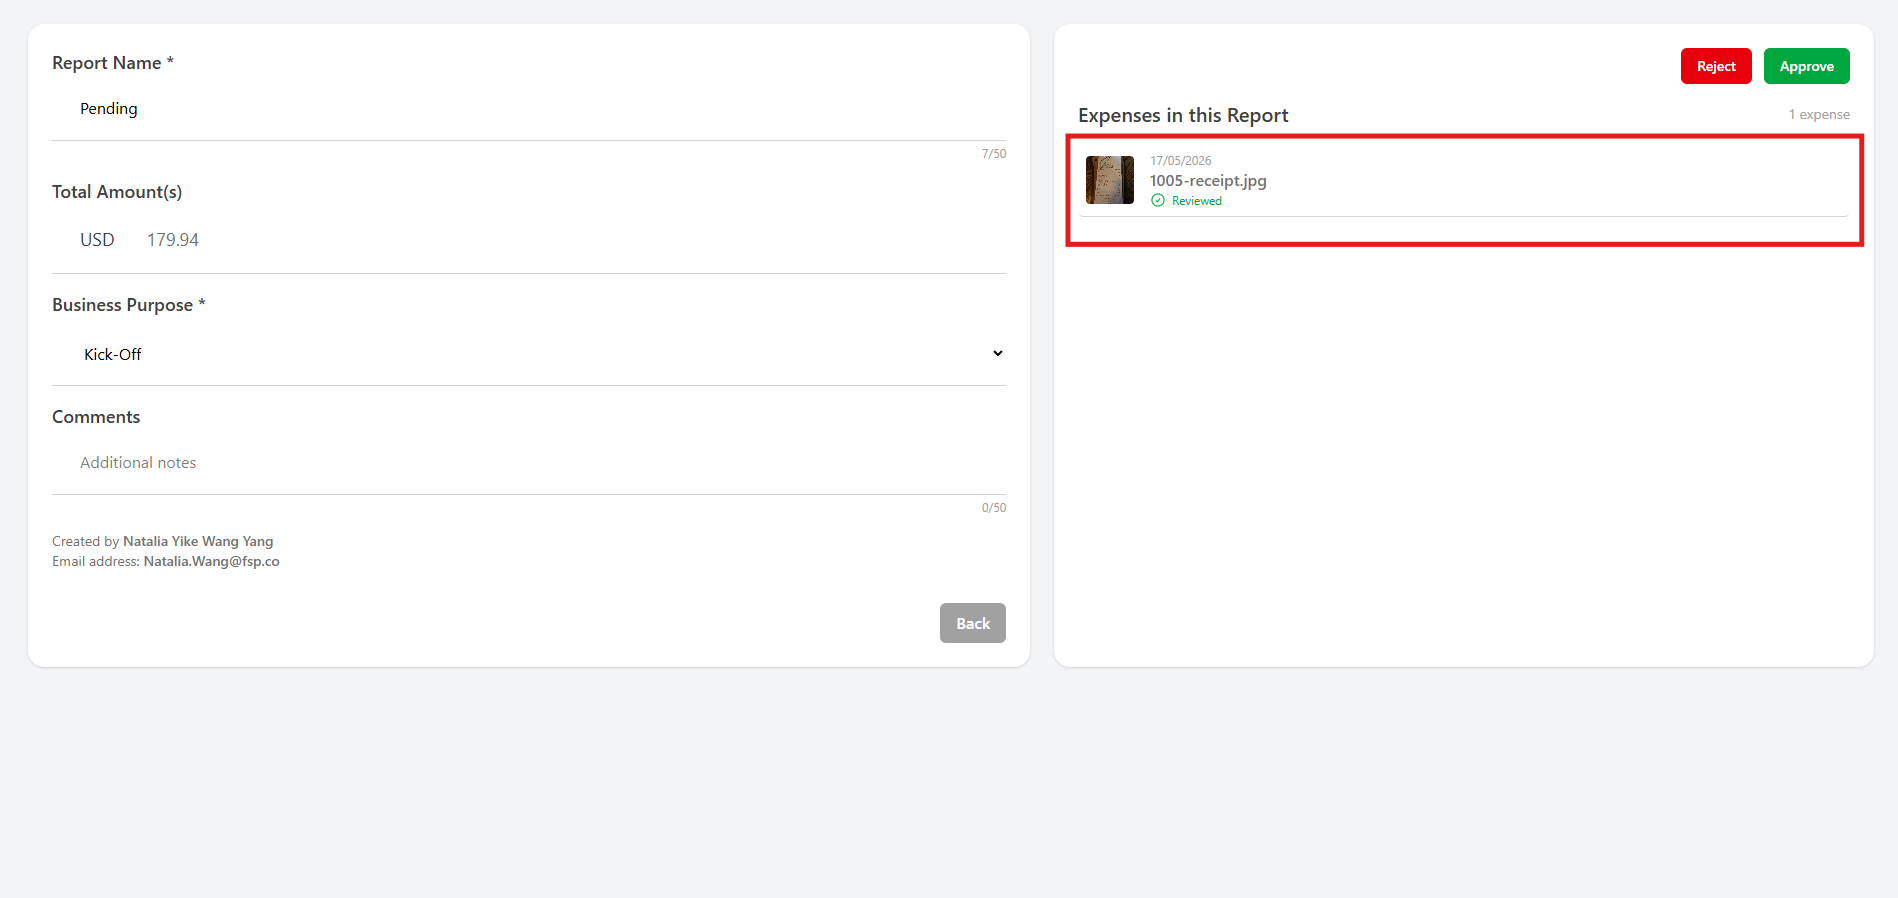
\includegraphics[width=0.8\textwidth]{Images/UserManual/image6.png}
        \caption[Report details view]
        {Report details view. [Own creation]}
        \label{fig:report-detail-information}
    \end{figure}

     After seeing the report details, click on any expense in the attached expenses list to review the expense details.
    
    \begin{figure}[H]
        \centering
        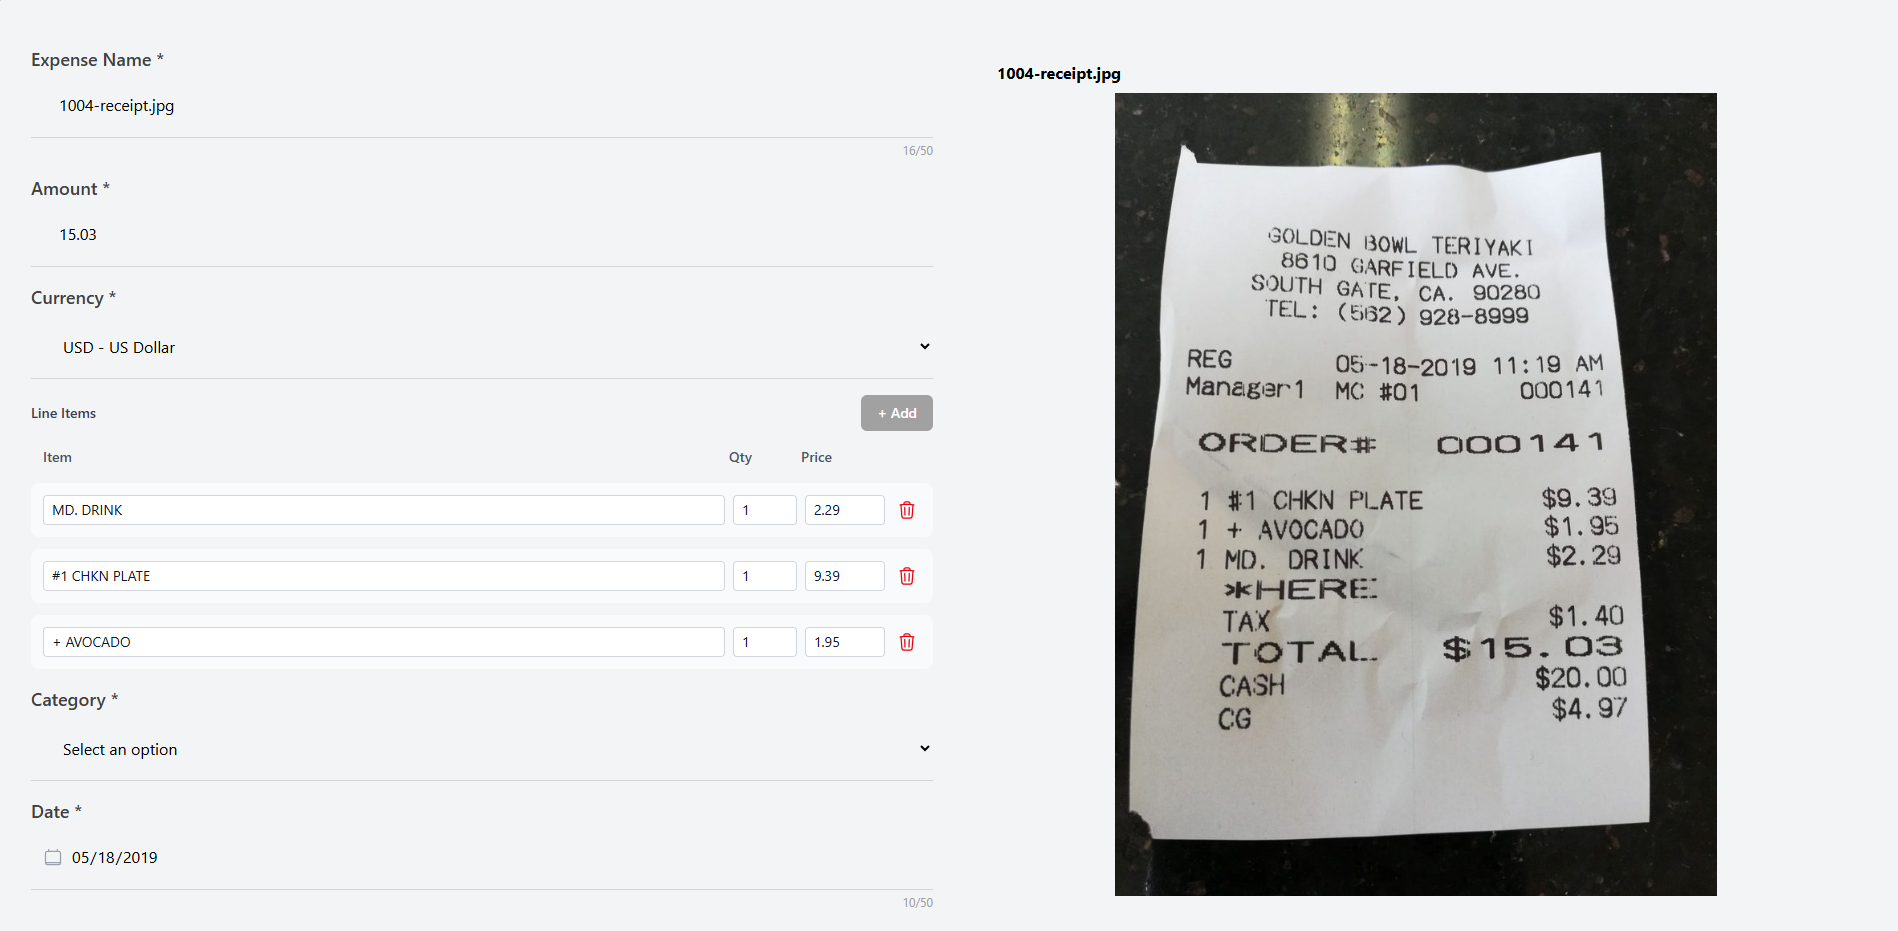
\includegraphics[width=0.8\textwidth]{Images/UIScreenshots/ExpenseInfoUpper.png}
        \caption[Expense details view]
        {Expense details view. [Own creation]}
        \label{fig:expense-details-view}
    \end{figure}

    Approve or reject the report by clicking the corresponding buttons in the report details view.


    \begin{figure}[H]
        \centering
        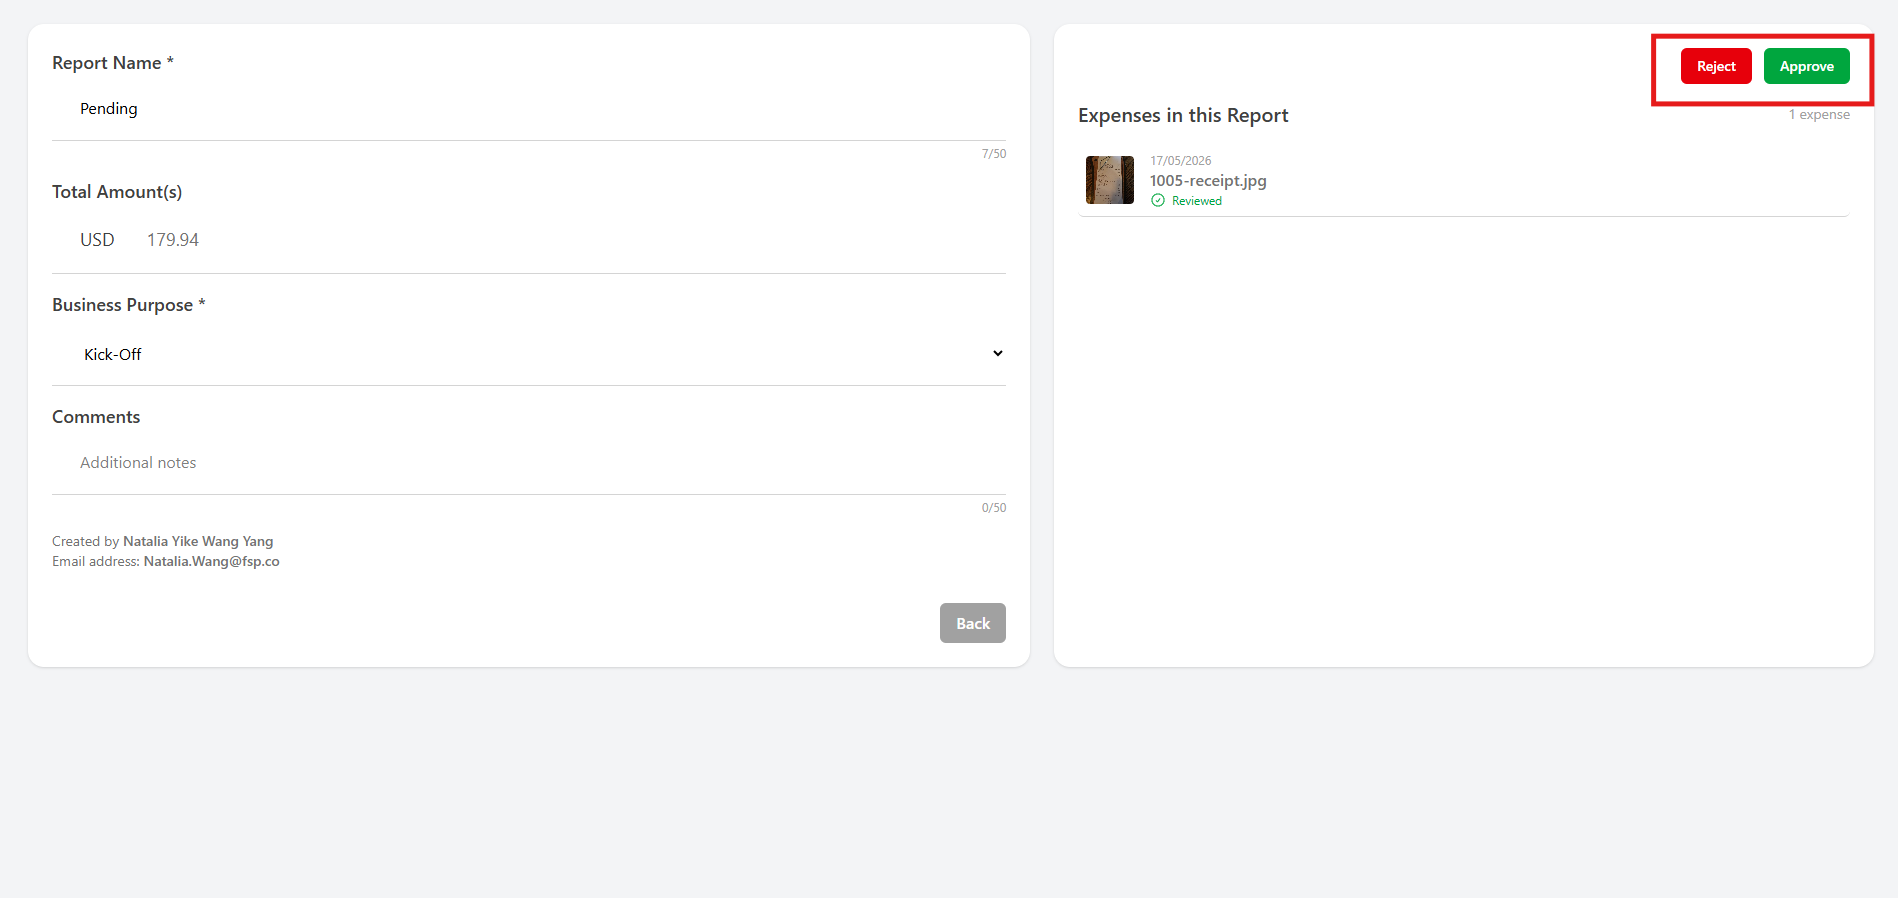
\includegraphics[width=0.8\textwidth]{Images/UserManual/image7.png}
        \caption[Approve or reject report buttons]
        {Approve or reject report buttons. [Own creation]}
        \label{fig:approve-reject-report}
    \end{figure}

    \item To view reports that have already been reviewed, select the \textit{Reviewed Reports} option from the upper screen tab.


    \begin{figure}[H]
        \centering
        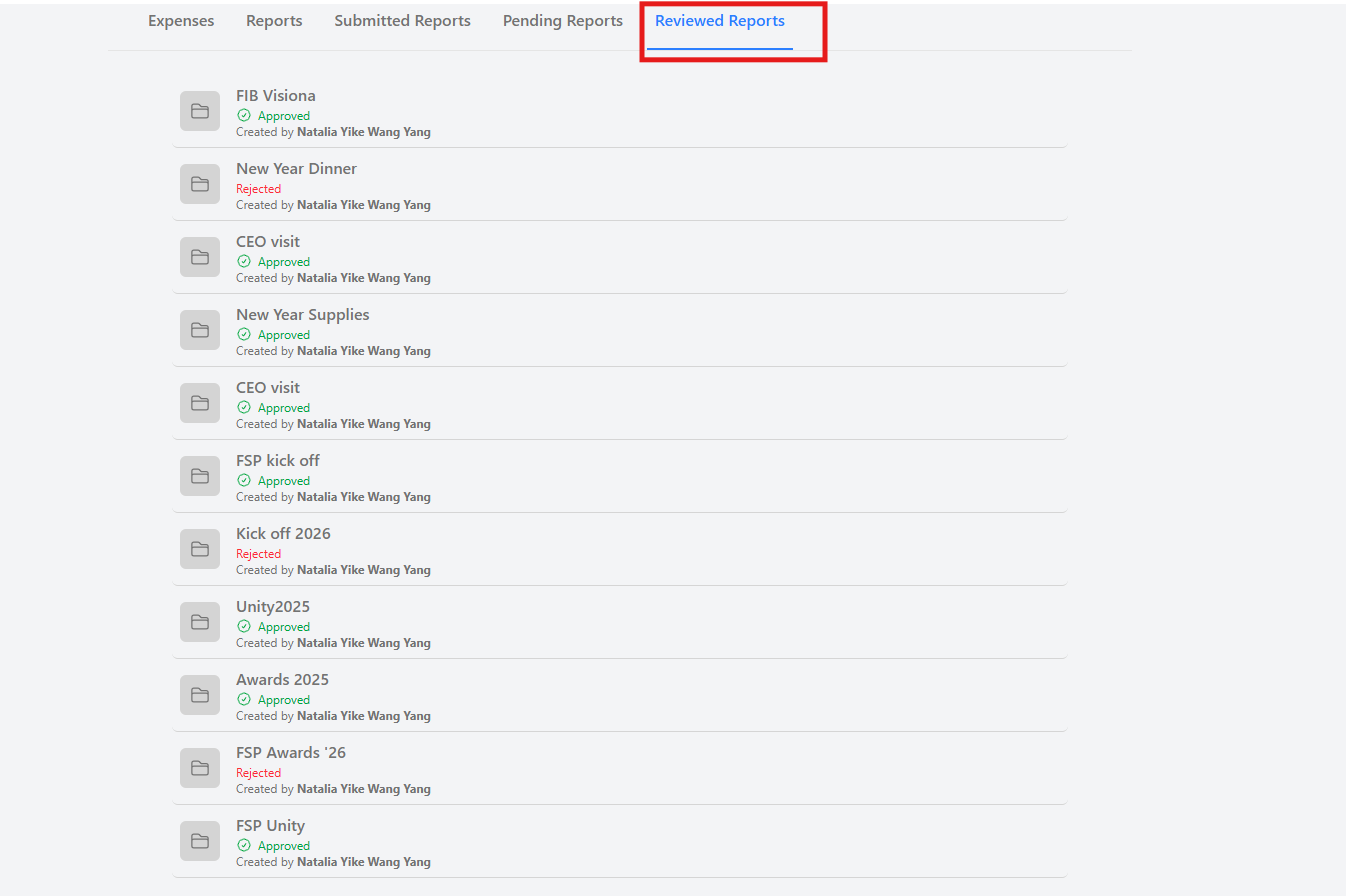
\includegraphics[width=0.8\textwidth]{Images/UserManual/image16.png}
        \caption[Reviewed Reports view]
        {Reviewed Reports view. [Own creation]}
        \label{fig:reviewed-reports}
    \end{figure}


    To view the report and their attached expense details, follow the procedure described in Step 2.

\end{enumerate}

